\section{Problem analysis}
\subsection{Internet of Things}
\subsubsection{Description}
The term "Internet of Things" was coined by Peter T. Lewis in September 1985 and covers the concept of connected physical objects enabled to exchange telemetry. The Internet, wireless communication and especially the Smart phone have made it possible to realize this, and is a growing and popular technology. 

\subsubsection{Concepts}
%Spime begrebet af Bruce Sterling
Characteristics to the Internet of Things is discussed by Bruce Sterling in his book "Shaping Things"\cite{books:shaping-things}, where he uses the word \textit{Spime} for objects which can be tracked through space and time (Sp-ime). The term was coined by Sterling and is a neologism for a "futuristic object" with these properties. He describes Spimes as something that can be created through six technologies: small inexpensive remote control, location awareness, data mining, virtual construction, rapid prototyping, and effective recycling. His idea of a Spime is an interesting concept in regard to the Internet of Things, as the concept very much can be realized in today's technological world through the Internet of Things.

Another neologism in the IoT language, which resembles Sterling's idea of a way to virtually construct an object, is the device "shadow". This is a concept heavily used to represent an object in the Cloud, and is used in all the IoT platform discussed in section \ref{iot_platforms}, but with different names. Having a virtual mirror of an object makes it possible to not depend solely on e.g. an object's Internet connection, as it can be synced with its shadow, when reestablished. 
%Device shadow

\subsubsection{Cloud-based computing}
What really makes IoT efficient and beneficial for a consumer is the property of a device to be always connected. This is realized through Cloud computing. Instead of relying on a storage device physically close to the object, having it connected to the Internet enables scalable real-time Cloud computing. 
%Hvor mødes IoT med dette?

The main characteristics and forces of Cloud computing is the resource usage and on-demand self-service. This has also been labeled "autonomic computing", while the "Cloud computing" refers to a distributed system that is distinguished from other systems through interconnection. In autonomic computing human intervention is reduced in the deployment of services, and the influence of the location of resources is diminishing compared to previous emerged distributed systems. In \cite[p. 4-5]{books:cloud-computing} the characteristics Cloud Computing are more formally described as follows:

\begin{enumerate}
	\item \textit{involves distributed computing resources and software services which instance number varies by adapting to unpredictable changes}
	\item \textit{performs a contextual behavior through methods of self-management, self-tuning, self-configuration, self-diagnosis, and self-healing}
	\item \textit{hides intrinsic complexity to operators and users, as implementing techniques for designing, building, deploying and managing computing systems with minimal human involvement and presents itself as a robust, fault tolerant and easy to manage and operate architecture and deployment}
\end{enumerate}

From point 1 it translates to a system being able to auto-scale, which is a very important feature in a large business with even thousands of customers. It also involves load-balancing, scheduling, and adaptive resource provisioning, which is the hardware aspect of it. Point 2 stands for actual self-maintenance and the ability to detect and act according to the environment and pre-defined policies. Point 3 addresses the importance of reliability, together with the property of easy deployment and minimal human involvement. One approach to deal with these applications is a platform-as-a-service (PaaS). Informally its definition states that it is a \textit{cloud computing model that delivers applications over the Internet} REF(http://searchcloudcomputing.techtarget.com/definition/Platform-as-a-Service-PaaS). What it is supposed to deliver is \textit{a Cloud-based approach that provides enterprises with all the functionalities for developing, deploying, and administering services, without the burden of installing, configuring, and managing the underlying middleware, operating system, and hardware} \cite[p. 9]{books:cloud-computing}. Examples of these in regards to IoT is further investigated in section \ref{iot_platforms}. 

\cite{books:big-data}

\subsection{Cloud based IoT platform}
\label{iot_platforms}
This section will investigate some of the big platforms for IoT cloud-based computing in order to be able to tell what they actually offer and how/if they differ in their product. 

\subsubsection{Google Cloud Platform}
\paragraph{Overview} 
\textit{Cloud Platform brings scale of infrastructure, networking, and a range of storage and analytics products you can use to make the most of device generated data.}\cite{website:gcp}
This is Google's own description of their IoT Cloud solution, and the references article is used for analysis in this section. \\

The platform can be divided into three basic components, the device, gateway, and cloud, each of which are characterized by the following: A \textit{device} is defined as hardware and software that directly interacts with the world, and are connected to a network and the Internet. A \textit{gateway} lets devices \textit{not} directly connected to the Internet reach a cloud service. The \textit{Cloud} is the \textit{endpoint} of device data, where it can be processed.\\

Several terms are used to describe what devices constitute, but the most important seems to be metadata and state information. Device metadata contains information such as ID and the date manufactured. The state information is basically the device status, such as "on"/"off". Furthermore devices must be associated with some security credentials for authentication. \textit{Telemetry} is the term for device data gathering, and is described as the \textit{eyes-and-ears data} the device collects in its environment. Once a device has been defined, telemetry can be sent to the Cloud Platform. As mentioned, a gateway can provide connection to the cloud, when e.g. protocol translation is needed. The Cloud Platform is the infrastructure for data management, which is depicted in figure \ref{fig:gcp:infrastructure}.

\begin{figure}[h!]
	\centering
	\includegraphics[width=0.7\textwidth]{figures/gcp/infrastructure.png}
	\caption{Diagram of the Google Cloud Platform IoT infrastructure}
	\label{fig:gcp:infrastructure}
\end{figure}

\paragraph{Services}
Google calls each of these components \textit{services}, and are categorized by their functionality and role in the infrastructure. Communication between the services are called \textit{pipelines}, which includes transforming, computing, combining, and moving data. The Cloud Platform also provides means for storing data in Google Firebase\cite{website:firebase}
and is especially used for continuously mirroring device states and exposing them to clients (See figure \ref{fig:gcp:firebase}).

\begin{figure}[h!]
	\centering
	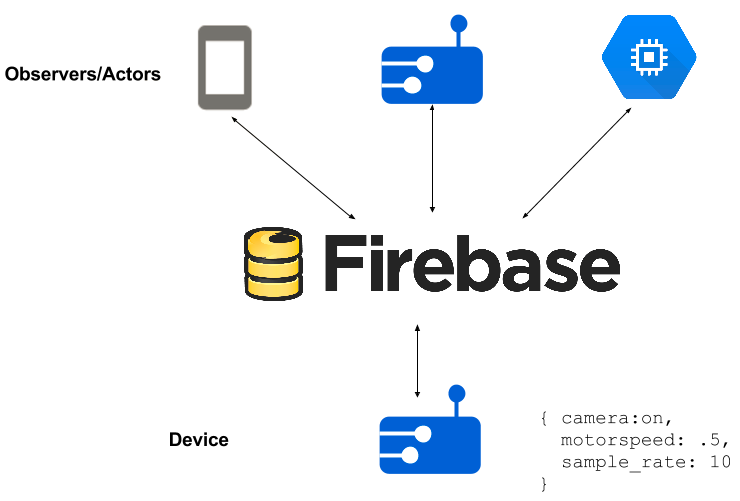
\includegraphics[width=0.5\textwidth]{figures/gcp/firebase.png}
	\caption{Abstract functionality of Google Firebase in the IoT Cloud Platform}
	\label{fig:gcp:firebase}
\end{figure}

The most interesting services are the "rule processing" and "streaming analytics", which allows for programmers to write custom logic for handling data triggered by device events. What you can do is to essentially trigger alerts, filter data, and invoke other APIs. This property of quick data processing is described as \textit{key} in the Cloud Platform. 

Google Cloud Platform is not just for IoT, but provides a plethora of products. Some of these can be utilized through integration with the Cloud Platform and include different storage services like Cloud SQL, data warehouse for analytics in BigQuery, data processing in Cloud Dataflow, as well as identity and access management in Cloud IAM.

Apart from the Cloud Platform, Google has created an Android-based IoT platform called "Android Things" (formerly known as "Brillo"), as well as a communication platform for IoT devices called "Weave". This has however not had much success and will not be investigated here.


\subsubsection{Amazon Web Services}
\paragraph{Overview} \textit{AWS IoT is a managed cloud platform that lets connected devices easily and securely interact with cloud applications and other devices.}\cite{website:aws}.
Aside from the huge and popular web shop Amazon hosts, they have developed a huge library of web services, called "Amazon Web Services" (AWS). Above citation is from their website and describes one of their products; The "AWS IoT Platform". \\

AWS IoT Platform constitutes of several components, labeled "AWS IoT Device SDK", "Device Gateway", "Authentication and Authorization", "Registry", "Device Shadows", and "Rules Engine". The infrastructure is depicted in figure \ref{fig:aws:infrastructure}. \\

\begin{figure}[h!]
	\centering
	\includegraphics[width=\textwidth]{figures/aws/infrastructure.png}
	\caption{Components of AWS IoT Platform and the infrastructure}
	\label{fig:aws:infrastructure}
\end{figure}

The \textit{AWS IoT Device SDK} provides software development kits to connect hardware devices or mobile applications, and supports C, JavaScript, and Arduino. Protocols like MQTT, HTTP, and WebSockets are supported for connectivity and data exchange. Furthermore Amazon has partnered up to offer a wider variety of SDKs, including Google's Android and Apple's iOS. The SDKs are meant for making integration with AWS easier for the programmer by encapsulating operations on the IoT Platform in library function calls. 

The \textit{Device Gateway} provides before mentioned protocols for communication between devices and the IoT Platform. It can be configured to work as a publication/subscription model for one-to-one and one-to-many communication, and it even scales automatically with \textit{over a billion} devices connected.

Security is taken seriously by Amazon, and this is what \textit{Authentication and Authorization} takes care of. Data between device and IoT Platform is never exchanged without proven identity, by use of "SigV4" and X.509 certificates. It's possible to fully manage mapping of authentication policies for connected devices, as well as revoking access rights at any time. Another feature is to use Amazon Cognito, which basically takes care of authentication for mobile applications.

The \textit{Registry} tracks device metadata by establishing unique identities for connected devices. 

\textit{Device Shadows} are persistent, virtual versions of connected devices and represent their sates. This allows for other devices to interact with other devices through a REST API. In other words, it is a convenient way of updates devices, as well as getting information about them. 

The data processing happens in the \textit{Rules Engine}, which evaluates messages passed to IoT Platform by user defined rules. The data can simply be transformed and passed to another device, or routed to other AWS cloud services for further processing. This includes several of the AWS services like AWS Lambda, S3, and DynamoDB. \\

Figure \ref{fig:aws:example} is an example of the IoT Platform and illustrates how a light bulb can controlled through above mentioned services. A mobile application sends instructions to a controller, which communicates with the IoT Platform in the cloud. Two rules are defined to act upon triggered events. One rule routes the data to other AWS services for evaluation, and the other changes the light color of the bulb. In either case the device shadow is updated with a new state. If the light bulb is turned off, requested device states are still saved in the device shadow.  
\begin{figure}[h!]
	\centering
	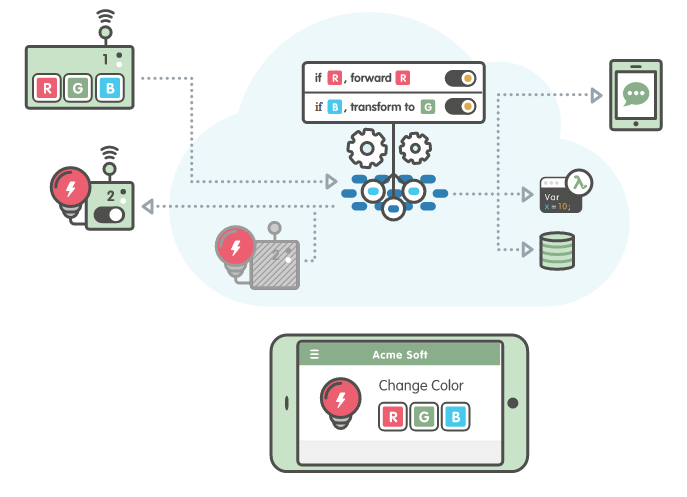
\includegraphics[width=\textwidth]{figures/aws/example.png}
	\caption{An AWS IoT Platform example illustrating the workings of the services.}
	\label{fig:aws:example}
\end{figure}

\paragraph{Services}
As mentioned in the overview, the Rules Engine allows for inbound data to be routed to other services. One worth mentioned is AWS Lambda, which executes computations in the cloud. It is even possible to write code in e.g. C\# and upload code snippets to the project. This service has the property of removing the need for a serer, as well as automatically scaling with the size of the workload. Other services like "DynamoDB" offers a NoSQL cloud database, and "Kinesis" for data analytics.  

\subsubsection{Microsoft Azure}
\textit{Azure IoT Hub is a fully managed service that helps enable reliable and secure bi-directional communications between millions of devices and a solution back end.} REF(https://docs.microsoft.com/en-us/azure/iot-hub/iot-hub-devguide)

Microsoft is another big player in the field of IoT Cloud computing, and offers their own IoT platform. Much confusingly they offer an IoT \textit{Suite}, as well as an IoT \textit{Hub}. The difference is that the IoT Suite is \textit{a collection of preconfigured solutions} REF(https://docs.microsoft.com/en-us/azure/iot-hub/iot-hub-what-is-azure-iot). This means that they have actually made customizable solutions based on common IoT scenarios, such as remote monitoring and asset management. The IoT Suite is however also the platform including the IoT Hub, which is the most important service in the IoT infrastructure, as it takes care of bidirectional connection with devices and the cloud. Figure \ref{fig:azure:infrastructure} illustrates the infrastructure of the platform from a device to the back end services. 

\begin{figure}[h!]
	\centering
	\includegraphics[width=\textwidth]{figures/azure/infrastructure.png}
	\caption{The Azure IoT Hub internal infrastructure.}
	\label{fig:azure:infrastructure}
\end{figure}


The IoT Hub keeps records of so called "Device twins", which are JSON documents containing device state and metadata information, for all connected devices. An identity registry enables devices to authenticate securely to the IoT Hub, which allows for full control of connecting devices. Devices communicate with the cloud though a device SDK or \textit{gateway}. The gateway is meant to be used when the offered SDKs do not support the device. Two types of gateways are offered, one being the \textit{protocol} gateway and the other being the \textit{field} gateway. The former is deployed in the cloud and performs protocol translation for MQTT, AMQP, and HTTP. The latter is deployed locally, i.e. physically close to the device(s), and enables also protocol translation, but also has the property of being able to actively manage devices, and the information mediated to the cloud. \\


\paragraph{Services}
Returning to the IoT Suite, a handful of services like Azure Stream Analytics, Storage, DocumentDB, Web Apps, and Power BI are available for integration with the IoT Hub. Together they provide means for data analytics, storage, visualization, and integration with back-office systems. REF(https://docs.microsoft.com/da-dk/azure/iot-suite/iot-suite-overview). Telemetry can be routed to an Azure service by user-defined rules in the IoT Hub, and requires no code. As mentioned the IoT Suite contains preconfigured solutions, which are labeled "Remote monitoring" and "Predictive maintenance". These solutions are the way to start building an IoT platform, and are customizable and extensible. 

\subsubsection{IBM Watson IoT}
\textit{Watson IoT Platform is designed to simplify cognitive IoT development so you can harness the full potential of the Internet of Things} REF(https://www.ibm.com/internet-of-things/).

IBM has a lot of different domain specific products and solutions in regards to IoT. They offer different solutions based on the business application, e.g. "Asset management", "Facilities management", and "Product development" REF(https://www.ibm.com/internet-of-things/iot-solutions/). They are all hosted on the IBM Bluemix cloud platform, which essentially is a big collection of offered products and services for cloud computing. One of them is the Watson IoT Platform, which provides a "powerful application access to IoT devices and data to help you rapidly create analytics applications, visualization dashboards, and mobile IoT apps" REF(https://console.ng.bluemix.net/docs/starters/IoT/iot500.html). The infrastructure of the platform is depicted in figure \ref{fig:ibm:infrastructure}.

\begin{figure}[h!]
	\centering
	\includegraphics[width=\textwidth]{figures/ibm/infrastructure.png}
	\caption{Infrastructure of the Bluemix service "Watson IoT Platform"}
	\label{fig:ibm:infrastructure}
\end{figure}


The Watson IoT Platform is described through six different concepts: organizations, devices, gateways, applications, events, and commands REF(https://console.ng.bluemix.net/docs/services/IoT/iotplatform\_overview.html\#about\_iotplatform). An organization is a way of separating systems and ensure data security through a unique identifier. This way, devices and applications are logically bound to a single organization and communication with other organizations can only happen with an explicit application for this purpose. Devices are divided into two classes; \textit{managed} and \textit{unmanaged} devices. The former contains a device management agent, which allows interactions with the Watson IoT Platform Device Management service. Such devices can perform operations which unmanaged devices cannot. This includes device management request and device management operations such as updates, downloads and reboots. Devices that cannot connect directly to the Watson IoT Platform can do so through a gateway. A gateway is both a device and an application that serves as an access point for other devices. Watson IoT Platform uses the HTTP and MQTT protocols for all communication. All devices and gateways must be registered in the Watson IoT Platform before they can connect to a service. Device manipulation and data interaction is controlled through applications, which do so with an API key and a unique application ID, all tied to a specific organization. Any application can subscribe to an event, which is triggered by a device and published to the Watson IoT Platform. Conversely, applications can communicate with devices through commands. The overall architecture of the Watson IoT is depicted in figure \ref{fig:ibm:architecture}, which resembles figure \ref{fig:ibm:infrastructure}, but is more elaborate

\begin{figure}[h!]
	\centering
	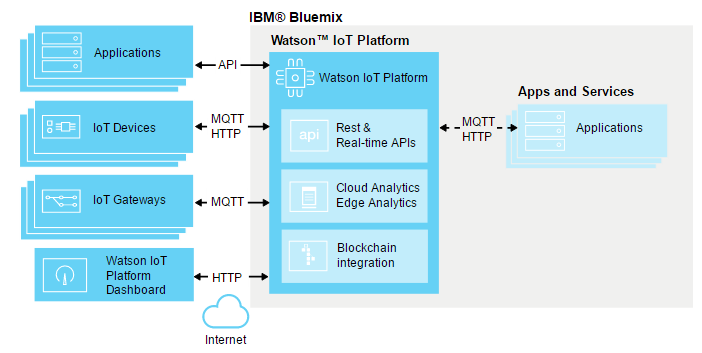
\includegraphics[width=\textwidth]{figures/ibm/architecture.png}
	\caption{Architecture of the Watson IoT platform}
	\label{fig:ibm:architecture}
\end{figure}

\paragraph{Services}
Watson IoT Platform provides a way of representing data set values of different devices in the GUI for a quick overview, through "boards and cards". Analytics rules are defines to specify the conditions that trigger actions. \textit{Cloud} rules trigger rules for devices connected directly to Watson IoT Platform, while \textit{edge} rules trigger rules for devices connected through gateways. Rules can trigger actions, which can be either of the following types: "Send email", "IFTTT"(Mentioned later), "Node-RED"(see below), "Webhook"(a means for altering a web page or application through callbacks). \\

Developing for Watson IoT Platform is supported by several SDKs and languages, such as C, C++, C\#, Node.js, and Java. Furthermore "Node-RED" is supported for the platform, which is an integrated visual tool to develop applications, devices, and gateways. \\

As Watson IoT Platform is one of the IBM Bluemix services, it can be integrated with other \textit{compatible} services that are hosted on Bluemix, e.g. for storage with "Cloudant NoSQL DB for Bluemix" or data to blockchain transactions with "Bluemix Blockchain" REF(https://console.ng.bluemix.net/docs/services/IoT/reference/extensions/index.html).

\subsubsection{External IoT services}
Apart from the big and popular IoT platforms investigated above, a lot of different IoT services exist, and some even effortlessly integrate with one another. Below, some are mentioned, and what they offer.
\paragraph{PubNub} offers a "Data Stream Network" for serverless device connections and message relaying.
\paragraph{IFTTT} stand for "If this then that", and is a rules engine for triggering actions through a variety of compatible systems, such as Philips Hue, and Weather Underground. REF(https://ifttt.com/about).
\paragraph{Cisco Jasper} provides an automated connectivity management with the "Control Center" to link devices to global networks and back-end systems. 
\paragraph{Oracle IoT Cloud Service} offers fast connection and integration with real time data analysis.

%Ved ikke om dette er relevant?

\subsubsection{Comparison}
This section will compare the four IoT platforms from Google, Amazon, Microsoft, and IBM, analyzed in the above sections. It is interesting to find out the differences and what they actually offer and for what purpose. First off a technical comparison can quickly give an overview of the specifications along some of the key features for an IoT cloud platform including the following:
\paragraph{Device management:} Keeping track of devices, their status and operations.
\paragraph{Integration:} Access to operations and data that needs to be exposed from the platform.
\paragraph{Protocols:} How data communication is transmitted. Important in regards to scalability.
\paragraph{Analytics:} The data collected from devices needs to be analyzed in some way.
The specifications to these parameters are illustrated in figure \ref{fig:tab:comparison}.

\begin{center}
	\rowcolors{1}{lightgray}{}
	\begin{tabular}{ | p{2cm} | p{2cm} | p{2cm} | p{2cm} | p{2cm} | }
		\hline
		IoT \newline Platform & Device \newline management & Integration & Protocols & Analytics \\ 
		\hiderowcolors
		\hline
		\cellcolor[gray]{0.9}
		Google Cloud \newline Platform & Firebase & REST API & HTTP, gRPC, \newline and gateway & Cloud Dataflow \\ 
		\hline
		\cellcolor[gray]{0.9}
		AWS IoT \newline Platform & Device Shadow & REST API & MQTT, HTTP, WebSocket, \newline and gateway & Amazon Kinesis, \newline AWS Lambda \\
		\hline
		\cellcolor[gray]{0.9}
		Microsoft Azure \newline IoT Hub & Device Twin & REST API & MQTT, AMQP, HTTP, \newline and gateway & Azure Stream \newline Analytics \\
		\hline
		\cellcolor[gray]{0.9}
		IBM Watson IoT & Dashboard & REST API & MQTT, HTTP, \newline and gateway & IBM IoT \newline Real-Time Insights \\
		\hline
	\end{tabular}
	\label{fig:tab:comparison}
\end{center}
REF(https://dzone.com/articles/iot-software-platform-comparison)
REF(https://blogs.endjin.com/2016/08/aws-vs-azure-vs-google-cloud-platform-internet-of-things/)

An important property of data analytics in IoT cloud computing is real-time behavior, which all of the above platforms offer. Apart from the different analytics services they offer, they differ in some of the communication protocols. Amazon, Microsoft, and IBM have adopted the popular MQTT protocol, while Google offers the "general RPC framework" (gRPC) with their Cloud Pub/Sub service. REF(https://cloud.google.com/pubsub/grpc-overview). All of them support the HTTP protocol through a REST API. 

When it comes to device management they all have some way of keeping statistics of registered devices. AWS uses "Device Shadow" as a virtual mirror of the device similar to Azure's "Device Twin". IBM uses the same concept and keeps a list of connected devices in the platform dashboard. Google on the other hand has no "real" integration of this concept, but uses the stand-alone Firebase service to maintain records of devices. 

With this said, the four platforms seem very identical, at least in regards to technical features. Using the platforms and reading their documentation however, they seem to have primary focus on different application domains. Azure for instance comes with two preconfigured IoT solutions directly aimed a business analytics and remote monitoring. AWS highlights the Lambda service together with the Rule Engine as one of the key features, making it possible to completely customize the cloud computed behavior. Watson IoT Platform focuses on application development and its integration with IoT, but offers different platforms for different needs, which is a design choice to not keep it all under same roof. Google seems to be a bit behind the others in regards to a full cloud IoT platform solution, but offers a real-time analytics service as the main feature together with the Cloud Platform.


\subsubsection{Platform and services}
The words "platform" and "services" have thus far been used interchangeably, but what is the actual difference in regards to this topic? TechTarget (REF(http://searchservervirtualization.techtarget.com/definition/platform)) defines it as \textit{any hardware or software used to host an application or service.} With this definition a platform could be anything from an operating system to a vending machine. What is actually offered from the cloud platforms are services for e.g. cloud computing, tracking, storing, and messaging, and the ability to integrate these with one another through the Internet. Another term "Platform as a service" (Paas) seems to fit quite well on this concept, as its definition states that it is a \textit{cloud computing model that delivers applications over the Internet} REF(http://searchcloudcomputing.techtarget.com/definition/Platform-as-a-Service-PaaS). This means that it is a platform, but as it is \textit{delivered} to the user, it is a service. Instead of having a in-house platform with an internal infrastructure offering different services, a PaaS provides this on the Internet as a single service.

\subsection{Alternatives}
%Hvad skal dette?